\section{EM Algorithm}
\label{sec:emalgorithm}

An elegant and powerful method for finding maximum likelihood solutions
for models with latent variables is the \emph{Expectation Maximization} 
	algorithm. The EM algorithm is an iterative process through two
	steps: an expectation step (E-step) and a maximization step (M-step). During the iterations, a sequence of model parameters ${\bf \theta^{0}}$
, ${\bf \theta^{1}}$, ...., ${\bf \theta^{*}}$ is generated where ${\bf \theta^{0}}$ is the initial parameter and ${\bf \theta^{*}}$ is the converged parameter when the algorithm terminates.

\subsection{E-step}
\label{subsec:estep}

Suppose we have a data set of RSSI observations at
the sniffers from the target device: ${\bf \overline{S}}$ = \{
${\bf {s}}^{0}$, ${\bf {s}}^{1}$,\ldots,${\bf {s}}^{M}$\}. The E-step
corresponds to finding the expected value of the latent or hidden component ({\bf
		x} and {\bf z}) values given the observed data  ${\bf \overline{S}}$ and the current parameter estimates.
Using this observation set and the current parameter estimates, we find out the posterior probabilities \textbf{(or responsibilities)} as follows. 
For each observation ${\bf {s}}^{l}$,
\begin{align}
& \pi_{({x_{j}}, {z_{k}})}^{l}  = p({x_{j}} = 1, {z_{k}} = 1 | {\bf{s}}^{l}) \\ 
& = \frac { p({x_{j}} = 1)p({z_{k}} = 1)p( {\bf {s}}^{l} | {x_{j}} = 1, {z_{k}} = 1)} {\ \sum_{p=1}^J \ \sum_{q=1}^{K} p({x_{p}} = 1) p({z_{q}} = 1) p( {\bf {s}}^{l} | {x_{p}} = 1, {z_{q}} = 1)} \nonumber \\ 
& = \frac { \upsilon_{j} \ \tau_{k} N({\bf {s}}^{l} | {\bf {\mu}}_{j,k}, {\bf {\sigma}}_{j,k})} {\sum_{p=1}^J \sum_{q=1}^K \left[\upsilon_{p} \tau_{q} N({\bf {s}}^{l} | {\bf {\mu}}_{p,q}, {\bf {\sigma}}_{p,q})\right]. } 
\end{align}

\noindent The posterior probability value $\pi_{({x_{j}}, {z_{k}})}^{l}$ can be viewed as the {\it responsibility} that component $({x_{j}}, {z_{k}})$ takes for explaining observation ${\bf {s}}^{l}$. We determine this measure of responsibility for each observation in the data set ${\bf \overline{S}}$.

\subsection{M-step}
\label{subsec:mstep}

The M-step of the algorithm corresponds to `maximizing the likelihood' of
the observed data. This leads us to re-estimating the parameters for the next iteration based on the posterior probabilities calculated in the expectation step of the algorithm:
\begin{align}
\upsilon_{j} = \frac { \sum_{l=1}^{M} \ \sum_{k} \pi_{({x_{j}}, {z_{k}})}^{l}} {M},
\end{align}
\begin{align}
\tau_{k} = \frac { \sum_{l=1}^{M} \ \sum_{j} \pi_{({x_{j}}, {z_{k}})}^{l}} {M},
\end{align}
\begin{align}
\mu_{i \ (j,k)} = \frac  { \sum_{l=1}^{M} \pi_{({x_{j}}, {z_{k}})}^{l} s_{i}^{l}} {N_{j,k}},
\end{align}
where
\begin{align}
{N_{j,k}} = \sum_{l=1}^{M} \pi_{({x_{j}}, {z_{k}})}^{l}.
\end{align}

The variance parameter can also be updated accordingly.

\subsection{Convergence of Log Likelihood}
\label{subsec:convergenceofloglikelihood}

\begin{figure}
\centering
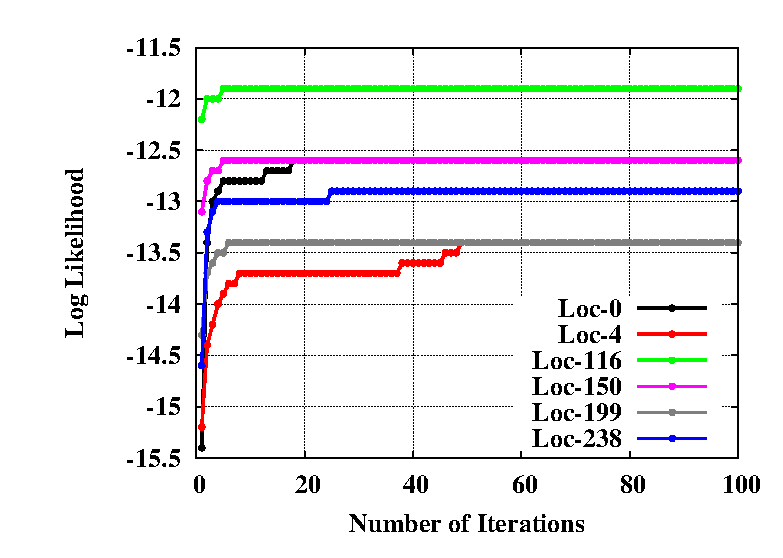
\epsfig{file=Figs4Paper/CEWIT/GMM-LogLikelihood/LogLikelihood.eps, height=1.5in, width=2.5in}
\caption{Convergence of log likelihood for 6 different instances of using GEM.}
\label{fig:loglikelihood}
\end{figure}

Each update of the parameters resulting from an E-step followed by an
M-step is guaranteed to increase the log likelihood function:
\begin{align}
\ln p({\bf \overline{S}} | {\bf \theta}) &= \sum_{l=1}^{M} \ln \left\{
\sum_{j=1}^J \sum_{k=1}^K \upsilon_{j} \tau_{k} \mathcal N ({{\bf {s}}^{l}} | {{\bf {\mu}}_{j,k}}, {{\bf \sigma}_{j,k}})\right\}.
\end{align}
The algorithm is deemed to have converged when the change in the log likelihood function falls below a threshold ($10^{-6}$ in the experiments described later).
Figure \ref{fig:loglikelihood} shows how the log-likelihood converges for six different instances of running GEM. Each instance here was to localize an android phone on the CEWIT testbed.



\subsection{Handling Identifiability}
\label{subsec:handlingidentifiabilityinourmodel}

There is an identifiability problem in this general approach that is well understood~\cite{Bishop:2006:PRM:1162264}. This arises because there are $P!$ equivalent solutions
in a $P$ component mixture model. In our case,
each component is a (location,
power-level) pair. 
We handle the problem of identifiability 
by using the knowledge of sniffer locations and initializing the EM algorithm
using the basic log-distance radio propagation model~\cite{Rappaport:2001:WCP:559977, Molkdar91} below:
%\subsubsection{Indoor Radio Propagation Model}
%\label{subsubsec:indoorradiopropagationmodel}
\begin{align}
P_r(d) = G\frac{P_t}{d^\alpha},
\end{align}
where $P_r(d)$ is the received power at distance $d$ and $P_t$ is the transmit power.
$\alpha$ is the path loss exponent which is simply a model parameter. 
In free space $\alpha =2$, but it typically increases somewhat in complex 
environments. $G$ is a frequency and antenna dependent constant. 
Often the above equation is expressed somewhat differently as: 
\begin{align}
P_r(d) = P_r({d_0}) - 10\alpha\log\left(\frac {\it d} {\it d_{0}}\right)
	\label{eqn:pathloss_1},
\end{align}
%\noindent
where $P_r$ is now expressed decibel (dB) units. This emphasizes that when powers 
are expressed in dB units
transmit power changes expressed in dB causes the same dB change at all receivers
regardless of location. In our experiments we will use RSSI in dB units. We independently
verified (not reported here for brevity) that the RSS measurement on our sniffer hardware is accurate at least to the extent
that a dB shift in the transmit power does get recorded as a similar
shift at the sniffer regardless of location.

\subsubsection{Initializing the components of our Model}
\label{subsubsec:initializingthecomponentsofourmodel}

In Equation \ref{eqn:pathloss_1},  $P_r({d_0})$ is the signal power at
some reference distance $d_{0}$ from the sniffer. This reference signal
strength $P_r({d_0})$ can be derived empirically or obtained from
wireless network hardware specifications \cite{Bahl00radar:an}. In our
deployment all our sniffers have the same hardware (described in detail
		in Section \ref {sec:evaluation} ) . The value of $P_r({d_0})$
was empirically found to be approximately 60 dB when $d_{0}$ = 1 meter . No assumption is made about the
target space, so $\alpha =2$. The path loss equation of equation
\ref{eqn:pathloss_1} can now be succintly expressed as: 
\begin{align}
P_r(d) = 60 - 10\alpha\log\left({\it d} \right)
	\label{eqn:pathloss_2},
\end{align}
 
For a location $L$ at a distance $d$ from a sniffer, equation
\ref{eqn:pathloss_2} gives us the theoretical RSSI value $P$ at the
sniffer. However, different devices may work at different power-levels
for doing wireless transmissions. Thus we generate $k$ values ranging from
$[P-\frac{k}{2} , P+\frac{k}{2}]$ to initialize the means for the $k$
component from location $L$. We do this procedure for every possible
target location in the map.  The standard deviation ($\sigma_{j, k}$)
	was chosen as 5 (and kept fixed to reduce computation time). This
	choice was mostly arbitrary though some previous work
	\cite{Tao:2003:WLL:941311.941314} also use fixed values of standard
	deviation ($\sigma=12$) in
	their work. 

\subsection{Final Location Estimate}
\label{subsec:finallocationestimate}

\begin{figure*}
	\centering
		\subfloat[CEWIT]{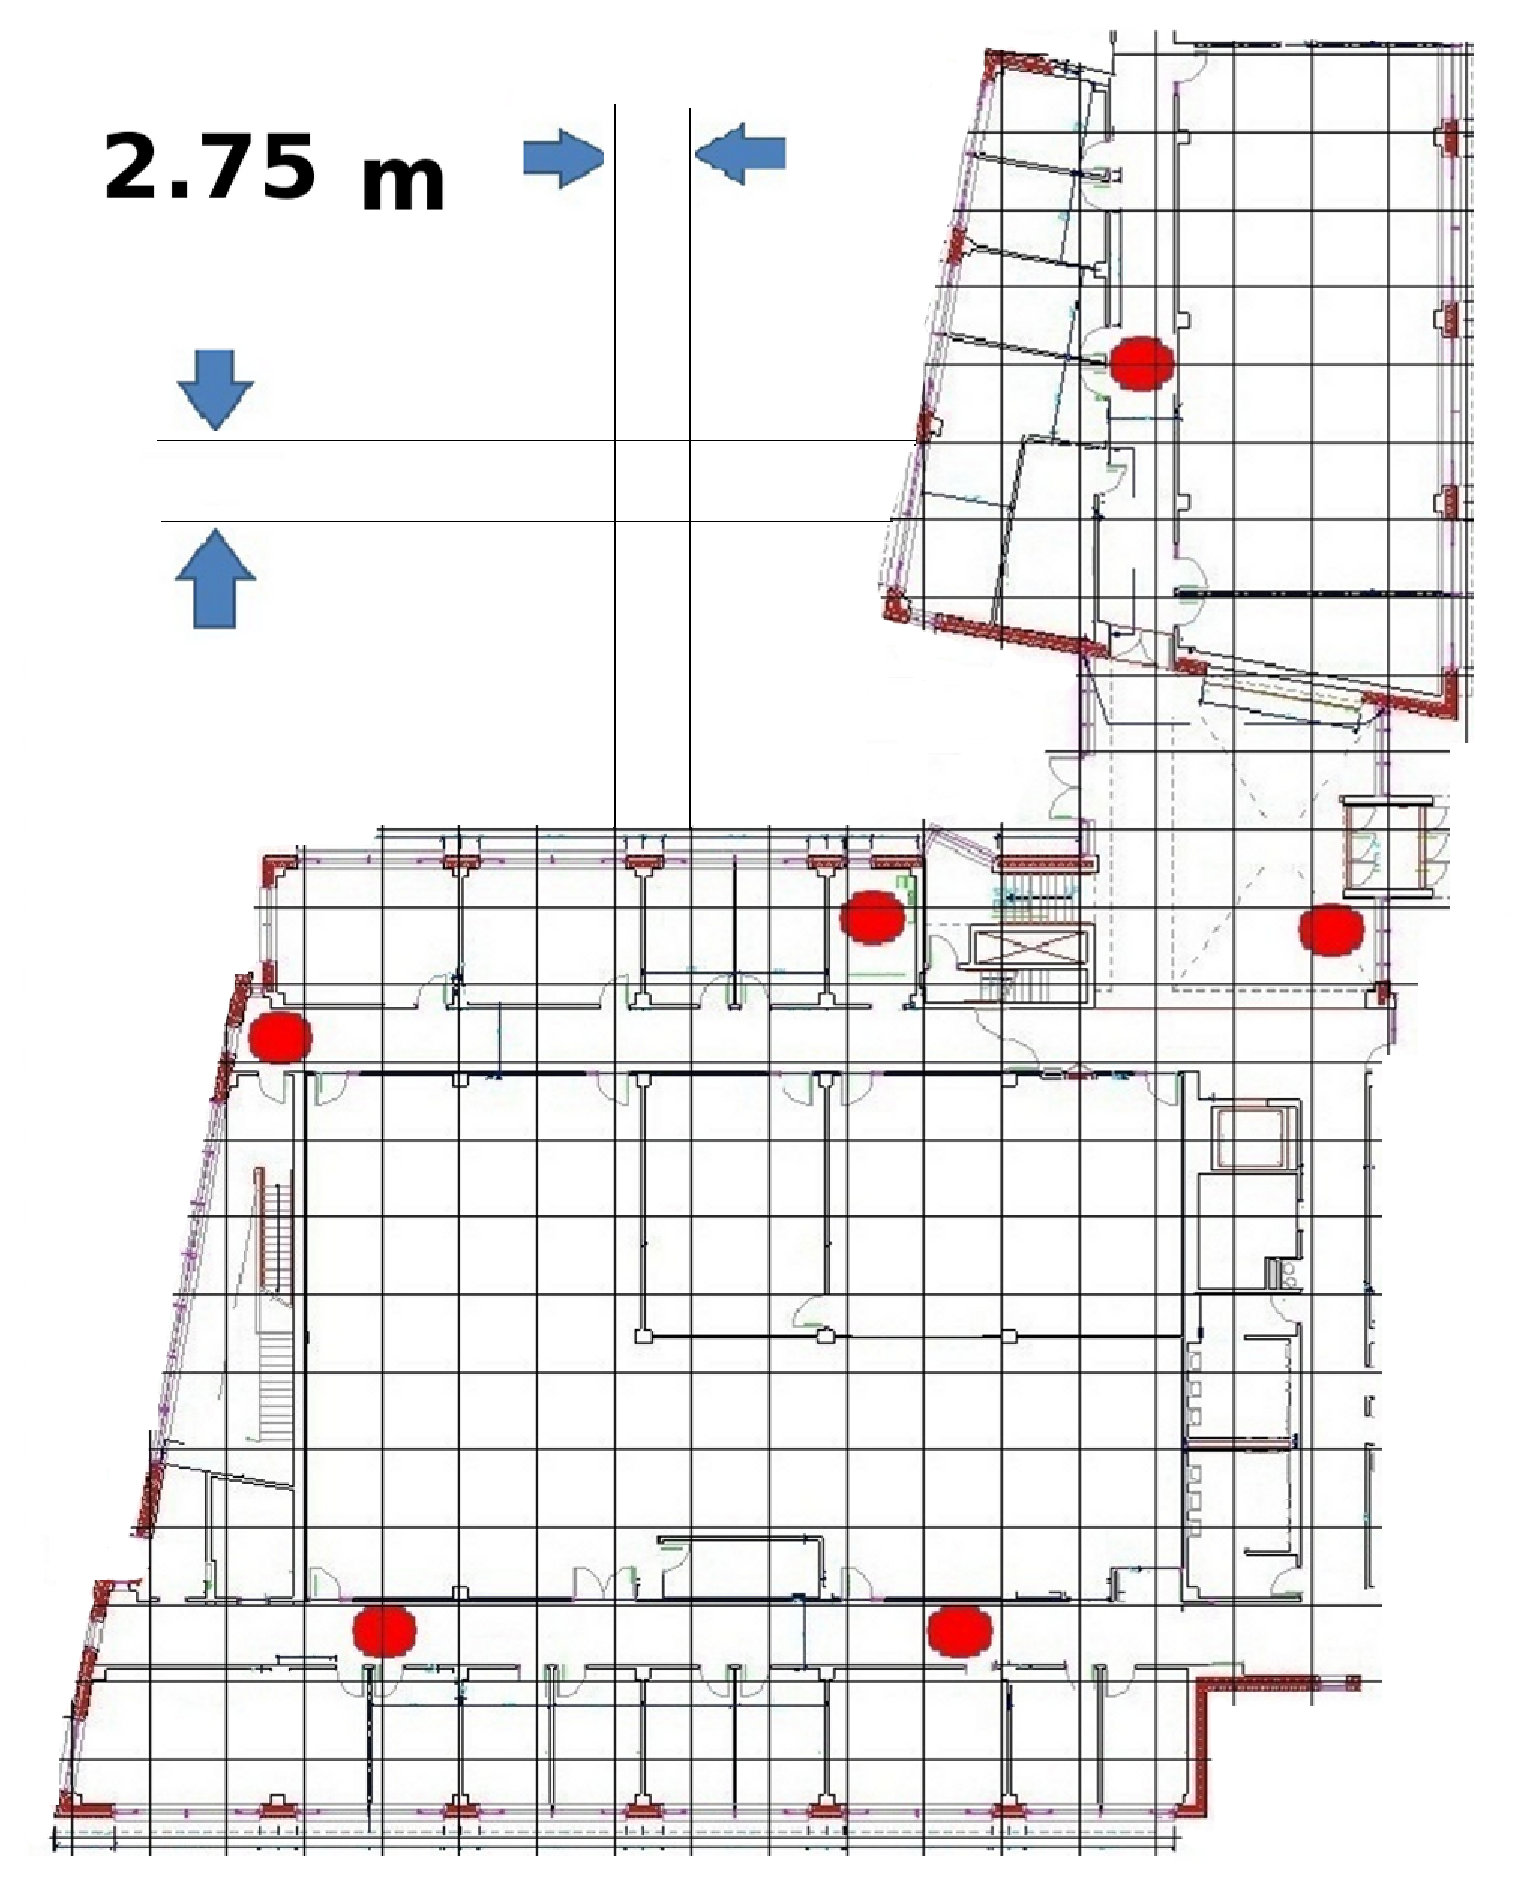
\includegraphics[height=2.5in, width=2in]{Figs4Paper/CEWIT/CEWIT-Map7.eps}} \quad \quad
		\subfloat[CSD]{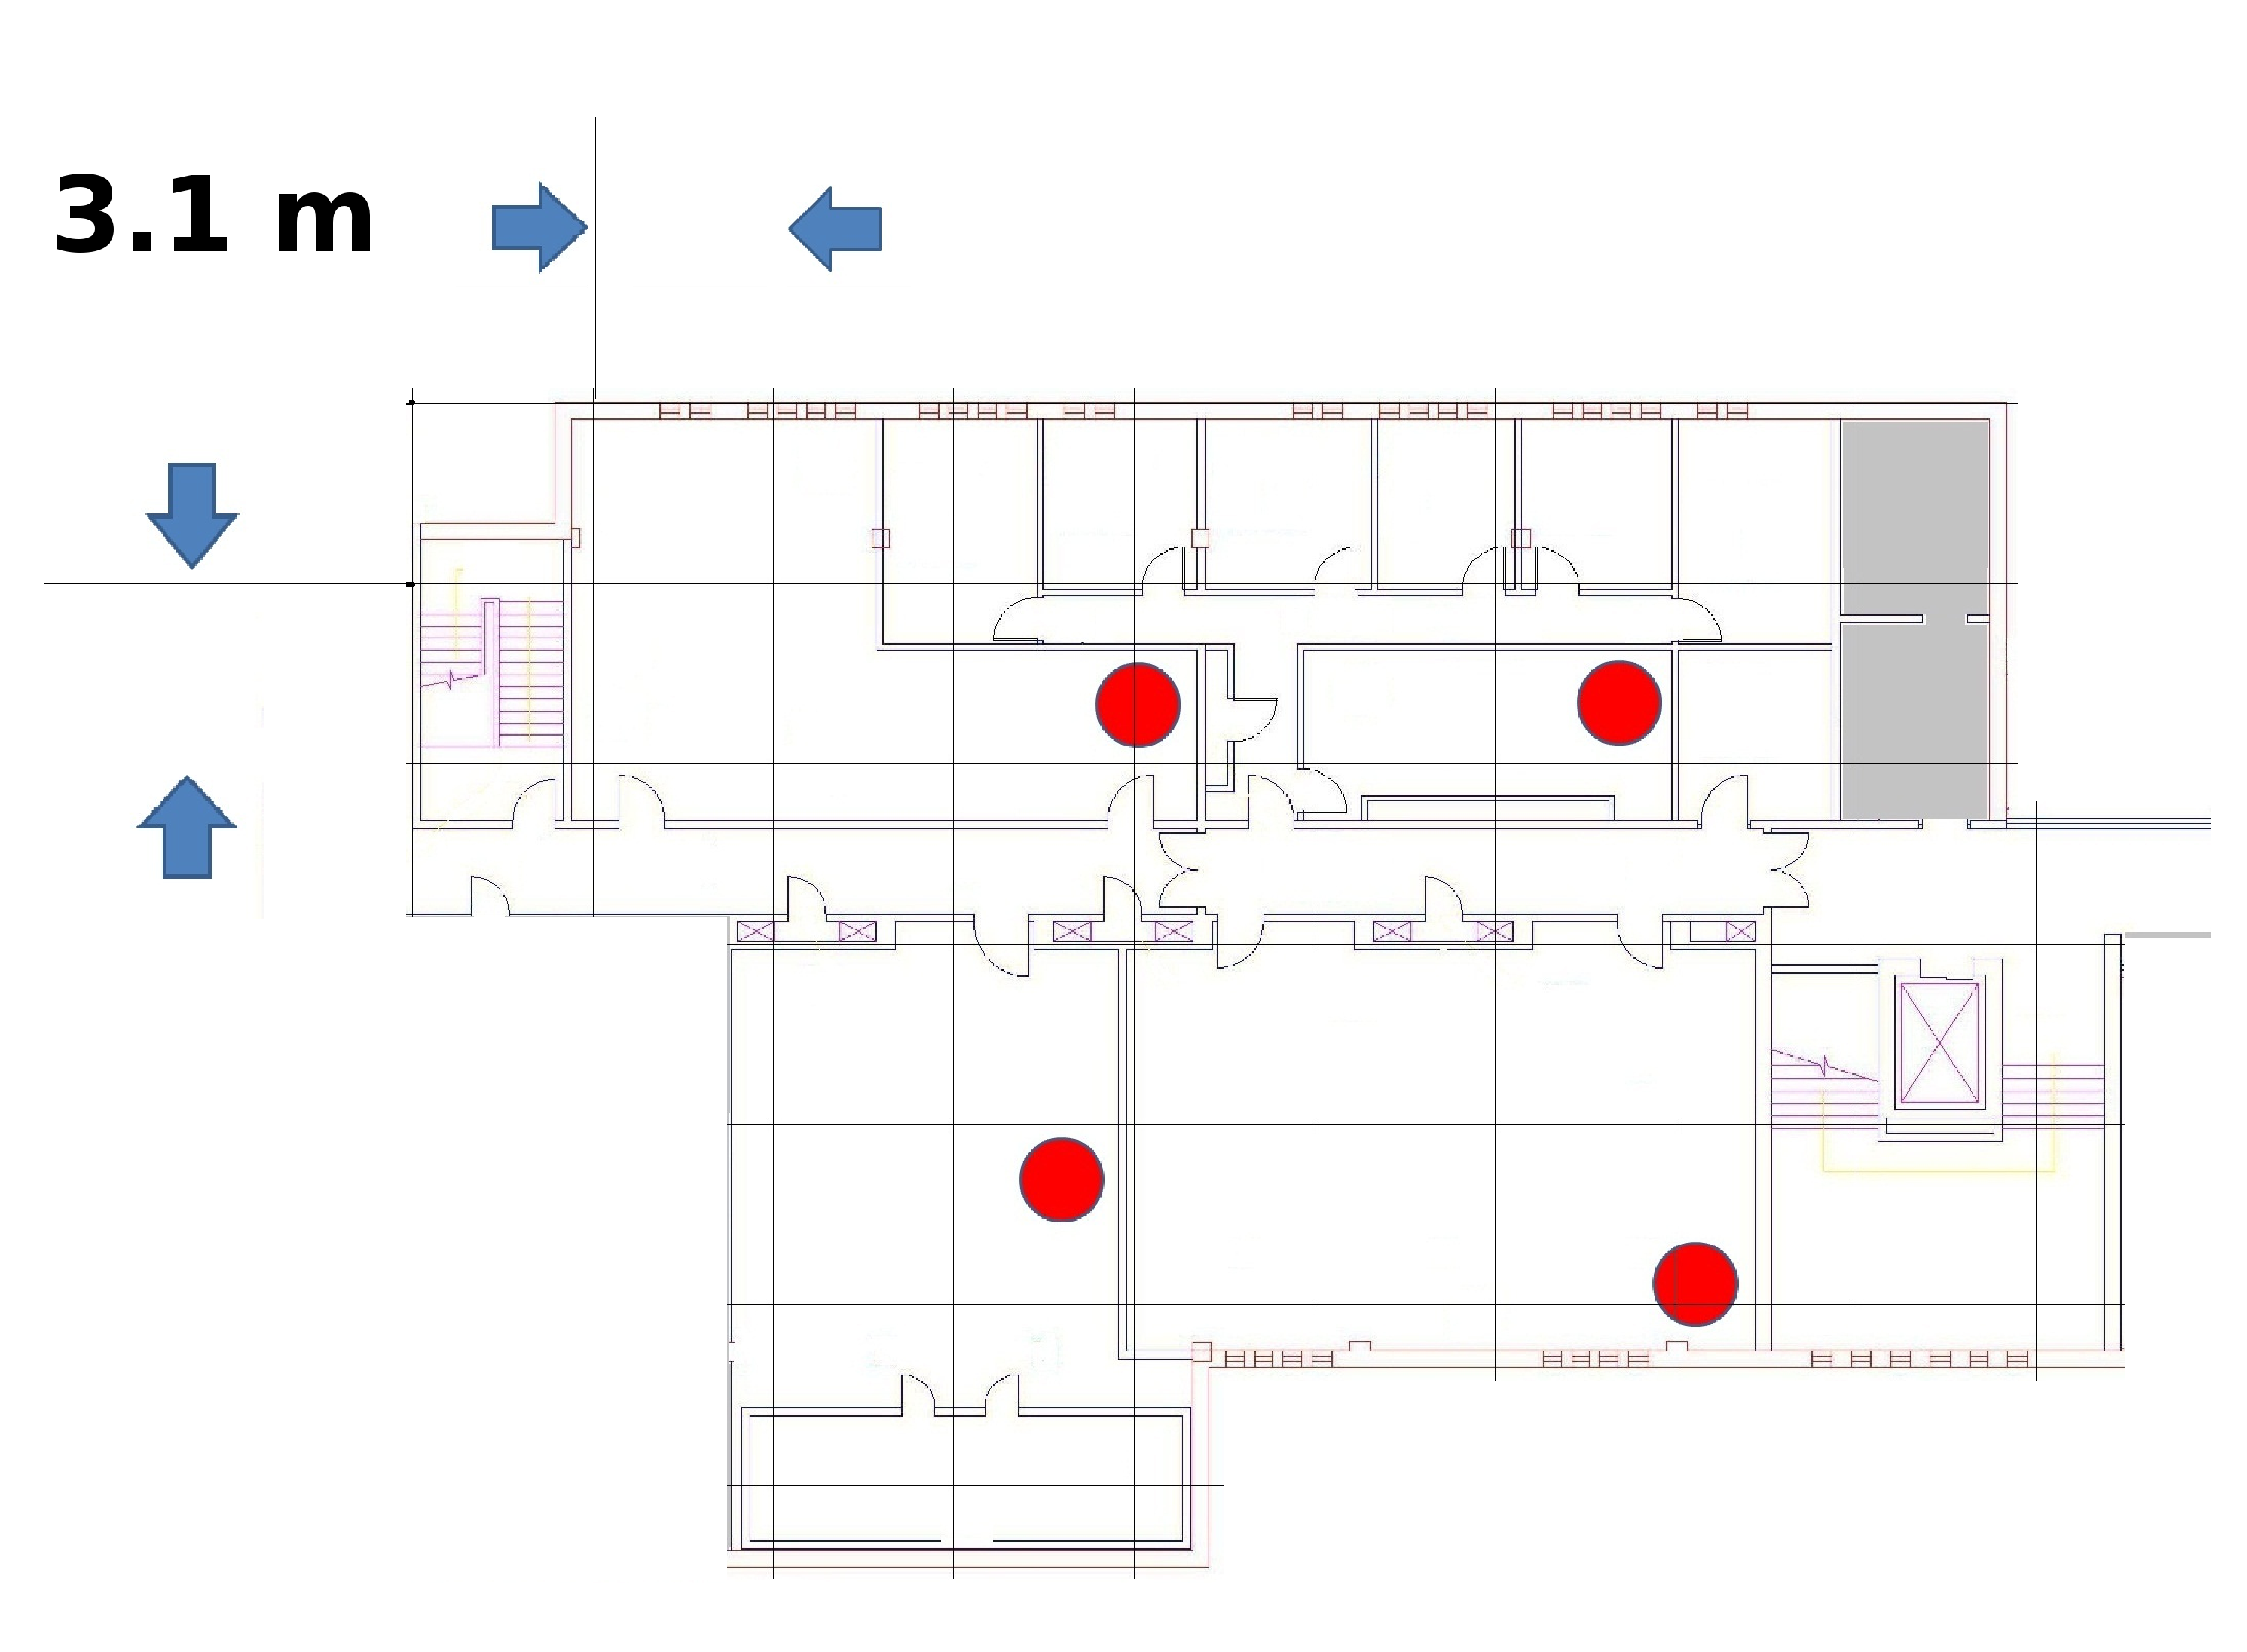
\includegraphics[height=1.5in, width=2.5in]{Figs4Paper/CSD/CSD-Map4.eps}} 
	\caption{Two testbeds for validation experiments. The red circles represent sniffer locations.}
	\label{fig:experimenttestbed}
\end{figure*}


Given a real-time received RSS vector ${\bf {s}}^{(obs)}$, we can now
find the location with the highest probability. We do this by first
finding the probability for each (location, power-level) pair and then
marginalizing over the power-levels. This gives us a probability
distribution over the possible locations inside the target space. The
location with the highest probability is returned as the answer.
Thus the estimated location index is given by $j^{*}$ where
\begin{align}
j^{*} = max_{j} \sum_{k} P({x_{j}} = 1, {z_{k}} = 1 | {\bf {s}}^{(obs)}) 
\end{align}
